
\section{Análise Léxica}
Esta etapa apresenta o desenvolvimento de tokenização do subconjunto do ambiente de equação do \LaTeX{}. A entrada para essa etapa são os caracteres do arquivo fonte, e a saída é uma organização lógica desses caracteres em sequencia que formam os \texttt{tokens}. O código dessa etapa se encontar no pacote \texttt{lexer} apresentado em \autoref{estrutura-de-pacotes}.

Primeiro, realizamos um laço sobre o arquivo inteiro, passado caracter à caracter para extrair os tokens. Antes realizamos uma checkagem de igualdade com a string
\verb|\begin{equation}| para decidir se já podemos começar a extrair os tokens. Dessa maneira permitimos que outros textos que não estão dentro da delimitação, a qual acaba com \verb|\end{equation}|, possa existir, como textos explicatorios dentro de um mesmo arquivo de extensão \texttt{.tex}.

Por conveniencia, apresentamos uma gramatica para geração dos \texttt{tokens}, escrito apenas para fins de documentação, \autoref{grammar-tokens}, o alfabeto dessa gramatica são os caracteres.
A geração de tokens internamente possui sua implementação similiar a simulação de uma máquina de estados.

Na definição da gramática (\autoref{grammar-tokes}), utilizamos uma notação leve de sintaxe para representá-la. Palavras com todas as letras minúsculas são não-terminais, enquanto palavras entre aspas simples representam literalmente \textit{caracteres} com esse conteúdo. Palavras em letras maiúsculas representam um um \textit{caractere} que pode variar, mas mantém o mesmo significado semântico. Por exemplo, \texttt{DIGIT} pode ser um digito de 0 à 9, mas nas regras de produção eles são tratados de maneira idêntica. LETTER é outro exemplo, que significa, uma letra \verb"a" à \verb"z". O símbolo ``$*$'' indica zero ou mais ocorrências, ``$()$'' indica agrupamento para aplicar um operador a ele, ``$|$'' simboliza o início de uma regra alternativa para o mesmo não-terminal, ou se estiver dentro de um agrupamento dessa maneira``$(a|b)$'' significa que aceita a ou b e ``$=$'' indica uma produção. Essa mesma definição de gramatica é utilizada para \autoref{grammar}, com a diferença que o alfabeto dela são formato pelo conjunto de tokens gerados nessa etapa.

O pacote inteiro pode ser chamada através de uma unica funcão, vista no \autoref{function-lex} em sintaxe \texttt{Odin}. Significa que temos um procedimento, chamado \texttt{lex} que aceita uma a lista de caracteres, e retorna uma lista do tipo \texttt{Token} (\autoref{lexer-structs}), esse tipo é uma estrutura que possui os campos: \texttt{kind}, que discrimina o tipo de token, que corresponde a uma das regras de produção na \autoref{grammar-tokens}; \texttt{text}, corresponde à string que o gerou; \texttt{position} instacia do tipo \texttt{Position}.

\begin{codigo}[htb]
        \caption{\small Função principal do Lexer. }
        \label{function-lex}
  \begin{lstlisting}[language = c]
  
    lex :: proc(input: []u8) -> []Token
  \end{lstlisting}
\end{codigo}

A medida que iteramos nesse \texttt{input}, também matemos algumas variaveis de controle, como contagem que quebra de linhas (\verb|"\n"| ou \verb|"\n\r"|), coluna atual e o cursor que reprenta index que aponta para o caractere sendo processado. A contagem de quebra de linha e coluna é importante para preencher a estrutura o campo do token correspondente ao tipo \texttt{Position}, representado em \autoref{lexer-structs}, que por sua vez é essencial para reportagem de errors. O reporte de erros que é implemnetada nessa etapa e utilizada por todos os pacotes do proejto, sua função possui possiveis assinatura vista no \autoref{function-errors}:
function-errors

\begin{codigo}[htb]
    \caption{\small Função de erro exposto pelo pacote \texttt{lexer}. }
        \label{function-errors}
\begin{lstlisting}[language=C++]
error_from_pos :: proc(pos: Position, msg: string, args: ..any)
error_from_token :: proc(token: Token, msg: string, args: ..any);
\end{lstlisting}.
\end{codigo}.

Dado um posição ou um \texttt{token} exibimos uma mesagem (\texttt{msg}) que é mostrado na tela do terminal com uma formatação que mostra exatamente onde está o erro, em vermelho. Extraindo as informações do token sabemos exatamente como sublinhar o erro, pois sabemos qual o nome do arquivo, linha, coluna, e cumprimeto do token que gerou o problema, possibilitando uma clara mensagem de erros exemplificado no erro sematnico de uso de indentificador não definido \autoref{analise-erros}, erro de @@ outros errros @@

\begin{figure}[H]
    \caption{\label{error-balanceamento} \small Erro de balanceamento de parentesis.}
    \begin{center}
        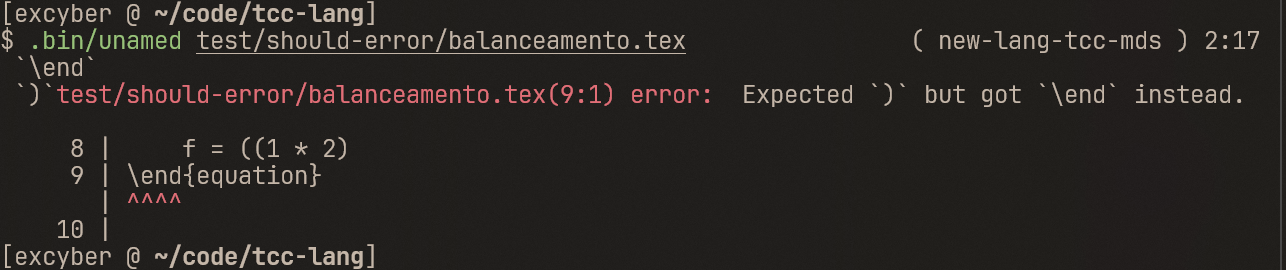
\includegraphics[scale=0.5]{./Imagens/error-balanceamento.png}
    \end{center}
\end{figure}

\begin{figure}[H]
    \caption{\label{error-reserved-word} \small Erro de @@@.}
    \begin{center}
        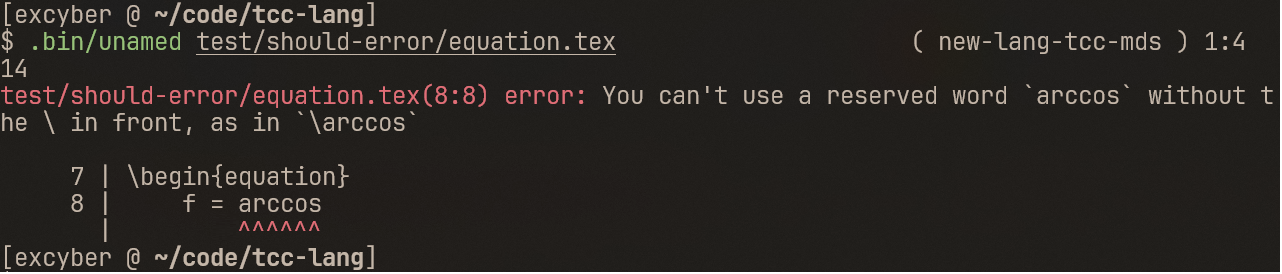
\includegraphics[scale=0.5]{./Imagens/error-reserved-word.png}
    \end{center}
\end{figure}

\begin{figure}[H]
    \caption{\label{error-incompatible-types} \small Erro de @@@.}
    \begin{center}
        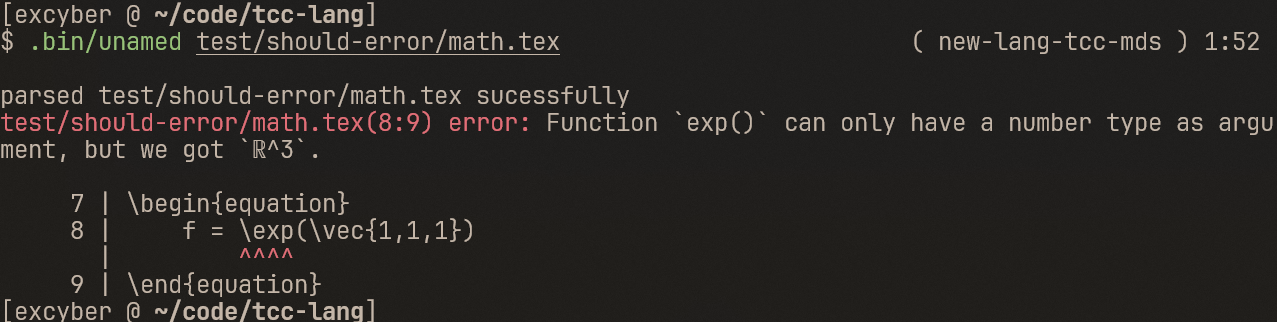
\includegraphics[scale=0.5]{./Imagens/error-incompatible-types.png}
    \end{center}
\end{figure}

\begin{figure}[H]
    \caption{\label{error-cant-make-expression} \small Erro de @@@.}
    \begin{center}
        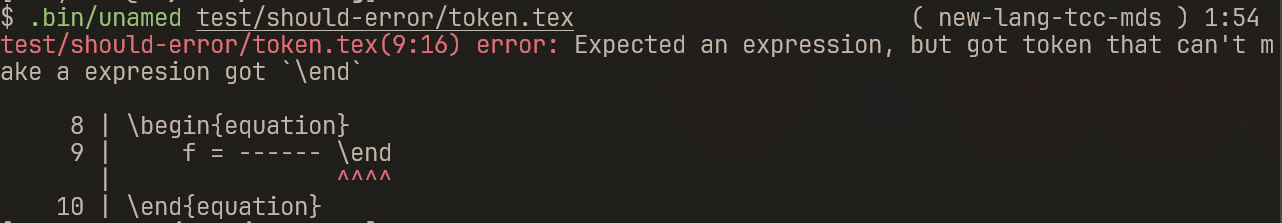
\includegraphics[scale=0.5]{./Imagens/error-cant-make-expression.png}
    \end{center}
\end{figure}

\begin{figure}[H]
    \caption{\label{error-undefined-symbol} \small Erro de @@@.}
    \begin{center}
        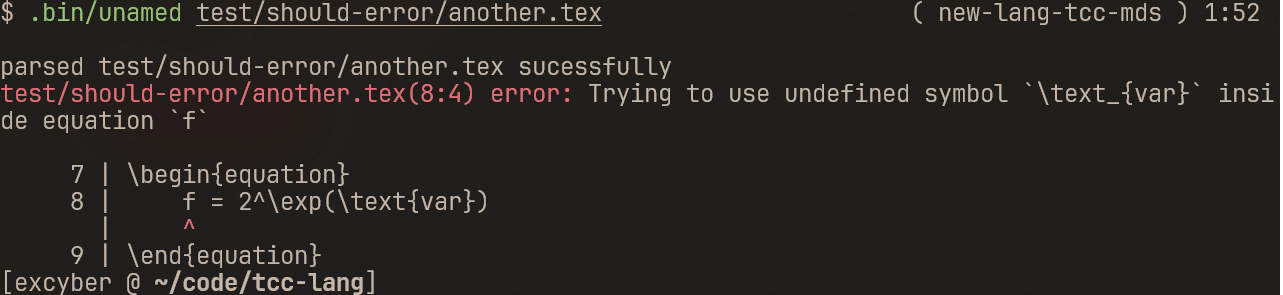
\includegraphics[scale=0.5]{./Imagens/error-undefined-symbol.png}
    \end{center}
\end{figure}

Tokens de um a dois caracteres são simples, basta ler um ou dois caracteres do input e contrtuir o token e continuar o laço até não poder mais. Se for ecnontrado o caractere \texttt{\%}, então o restante dos caracteres são ignorates até encontrar uma quebra de linha, isso é feito para dar supporte à comentarios \LaTeX{}.
Se for encontrado um digito ou letra então são classificados como indentificadores, números ou tokens especiais.

Numberos podem opcionalmente ter \. (ex: $1.0$). Indentificadores são formados por uma ou mais letras com o simbolo \verb"\" opcionalmente prefixo ao mesmo. Note que a grammatica de tokens é ambigua, uma sequencia de caracteres como \verb"\frac" pode ser interpretada como indetificar, para desmabiguar, criamos uma dicionário que mapeia um string à um token considerado esperial. Assim se o indetificador começar com o caractere \verb"\", mapeamos ele para um token especial através do dicionário exposto em \autoref{map-special-identifiers}.

Com laços represenmos a extração de.

Note que identificadores não permite numeros nem mesmo @underline ``\verb|_|'', pois  no analisador sintático, um nó do tipo indentificador é modelado como tipo recursivo, osi dentificadors podem ser aninhados, ao  conter outro nó. Sendo assim, não é necessario que ao nível de token seja permitido o underline em identifcador, isso permite indentificadores mais complexos a serem escritos como \verb|\pi_{n_1}| (renderizado em \LaTeX{} \ resulta em $\pi_{n_1}$). \verb"\pi"  seria o primeiro token do nó identificador e sua subexpresão seria \verb"n_1" ($n\_1$) que por sua vez é o identificador \verb"n" com subexpressão \verb"1".


\begin{codigo}[htb]
        \caption{\small Estuturas do Lexer. }
        \label{lexer-structs}
  \begin{lstlisting}[language=C++]

Token :: struct {
    kind: Token_Kind,
    val: union{i64,f64},
    text: string,
    pos:  Position,
}

/*
 .  Line and colum in the source string,
 .  we only store the end line and col position for simplicity
*/
Position :: struct {
    file:   string,
    offset: i64,   // starting at 0, buffer offeset in file
    line:   i64,   // starting at 1, starting
    column: i64,   // starting at 1
    length: int    // how much chars foward
}
    
  \end{lstlisting}
\end{codigo}


\begin{codigo}[htb]
        \caption{\small Mapa de indentificadores especiais. }
        \label{map-special-identifiers}
  \begin{lstlisting}[language=C++]

SPECIAL_WORDS := map[string]Token{
    "text"  = Token{text = "\\text",    kind =.Text},

    // Special
    "frac"   = Token{text = "\\frac",   kind =.Frac},
    "vec"    = Token{text = "\\vec",    kind =.Vec},
    "cdot"   = Token{text = "\\cdot",   kind =.Mul},
    "begin"  = Token{text = "\\begin",  kind =.Begin},
    "end"    = Token{text = "\\end",    kind =.End},
    "rho"    = Token{text = "\\rho",    kind =.Rho},
    "sqrt"   = Token{text = "\\sqrt",   kind =.Sqrt},
    "omega"  = Token{text = "\\omega",  kind =.Omega},

    // Cross product
    "times"  = Token{text = "\\times",  kind =.Cross},

    "max"    = Token{text = "\\max",    kind =.Max},
    "min"    = Token{text = "\\min",    kind =.Min},
    "exp"    = Token{text = "\\exp",    kind =.Exp},

    "cos"    = Token{text = "\\cos",    kind =.Cos},
    "sin"    = Token{text = "\\sin",    kind =.Sin},
    "tan"    = Token{text = "\\tan",    kind =.Tan},

    "arccos" = Token{text = "\\arccos", kind =.ArcCos},
    "arcsin" = Token{text = "\\arcsin", kind =.ArcSin},
    "arctan" = Token{text = "\\arctan", kind =.ArcTan},

    "theta"  = Token{text = "\\theta",  kind =.Theta},
    "phi"    = Token{text = "\\phi",    kind =.Phi},

    "alpha"   = Token{text = "\\alpha",      kind =.Alpha},
    "beta"    = Token{text = "\\beta",       kind =.Beta},
    "sigma"   = Token{text = "\\sigma",      kind =.Sigma},
    "pi"      = Token{text = "\\pi",         kind =.Pi},
    "epsilon" = Token{text = "\\epsilon",    kind =.Epsilon},

}

    
  \end{lstlisting}
\end{codigo}


\begin{codigo}[htb]
    \caption{\small Gramatica ilustrativa para \texttt{tokens}. }
        \label{grammar-tokens}
  \begin{lstlisting}[numbers=none, frame=none, language=haskell]

    token_number     = DIGIT DIGIT* '.' DIGIT DIGIT* | DIGIT DIGIT*;
    token_identifier = '\' LETTER LETTER* | LETTER LETTER*;
    token_cmpgreater = '>';
    token_cmpless    = '<';
    token_cmpequal   = '==';
    token_equal      = '=';
    token_mul        = '*' | '\cdot';
    token_cross      = '\times';
    token_div        = '/';
    token_plus       = '+';
    token_minus      = '-';
    token_caret      = '^';
    token_semicolon  = ';';
    token_comma      = ',';
    token_colon      = ':';
    token_question   = '?';
    token_bang       = '!';
    token_openparen  = '(';
    token_closeparen = ')';
    token_opencurly  = '{';
    token_closecurly = '}';
    token_tilde      = '~';
    token_underline  = '_'; --- @@@ used for subexpresions
    token_arrow      = '->';
    token_begin      = '\begin';
    token_end        = '\end';
    token_frac       = '\frac';
    token_vec        = '\vec';
    token_omega      = '\omega';
    token_theta      = '\theta';
    token_phi        = '\phi';
    token_rho        = '\rho';
    token_alpha      = '\alpha';
    token_beta       = '\beta';
    token_sigma      = '\sigma';
    token_pi         = '\pi';
    token_epsilon    = '\epsilon';
    token_max        = '\max';
    token_min        = '\min';
    token_exp        = '\exp';
    token_tan        = '\tan';
    token_sin        = '\sin';
    token_cos        = '\cos';
    token_arctan     = '\arctan';
    token_arcsin     = '\arcsin';
    token_arccos     = '\arccos';
    token_sqrt       = '\sqrt';
    token_text       = '\text';
    token_eof        = EOF;
    
  \end{lstlisting}
\end{codigo}


Um enumeração que representa o tipo de token é mostrada no \autoref{enum-token-kind}, cada entrada nessa enumeração é correspondente as regras de produção na gramatica apresentada em \autoref{grammar-tokens}. Ao lado direito de cada entrada aprensetamos o simbolo que o representa em comentarios.

\begin{codigo}[htb]
\caption{\small Enumeração dos tipos de \texttt{tokens}. }
    \label{enum-token-kind}
\begin{lstlisting}[language = C++]
  Token_Kind :: enum {
    EOF           = 0,
    Number,
    Identifier,

    Equal,        // =
    Mul,          // * ou \cdot
    Cross,        // X
    Div,          // /
    Plus,         // +
    Minus,        // -
    Caret,        // ^
    Comma,        // ,
    Colon,        // :
    Question,     // ?
    Bang,         // !
    OpenParen,    // (
    CloseParen,   // )
    OpenCurly,    // {
    CloseCurly,   // }
    Tilde,        // ~
    Underline,    // _
    Arrow,        // ->

    Begin = 256,  // \begin
    End,          // \end

    Frac,         // \frac
    Vec,          // \vec

    Omega,        // \omega
    Theta,        // \theta
    Phi,          // \phi
    Rho,          // \rho
    Pi,           // \pi
    Epsilon,      // \epsilon
    Alpha,        // \alpha
    Beta,         // \beta
    Sigma,        // \sigma

    Max,          // \max
    Min,          // \min
    Exp,          // \exp
    Tan,          // \tan
    ArcTan,       // \arctan
    Sin,          // \sin
    ArcSin,       // \arcsin
    Cos,          // \cos
    ArcCos,       // \arccos
    Sqrt,         // \sqrt

    Text,         // \text
    Invalid
}

\end{lstlisting}
\end{codigo}
